%!TEX root = ../Documentazione.tex
%%--------------------------------------------------------------------------
%% DATABASE
%%--------------------------------------------------------------------------



\chapter{Database}

\section{Struttura}
\label{structure}
Il database SQLite è stato implementato tramite SugarORM, un ORM (Object-Relational Mapping) sviluppato appositamente per Android. In questo modo le entità del database sono direttamente mappate su classi Java, utilizzando il pattern DAO (Data Access Object).\\
Il database contiene 5 entità all'interno del package \\\code{it.gbresciani.legodigitalsonoro.model}:
\begin{description}
	\item[\code{Word}] Contiene la parola, sia in italiano sia in inglese, e le sillabe che lo compongono.
	\item[\code{Syllable}] Contiene la sillabla e l'esadecimale del colore associato.
	\item[\code{WordStat}] Permette di tracciare il momento in cui una parola viene trovata.
	\item[\code{GameStat}] Contiene le statistiche di una particolare partita
\end{description}
In figura \ref{fig:entities} sono riportati dettagli delle entità.

\begin{figure}[h!]
\label{fig:entities}
  \centering
    \centering{
      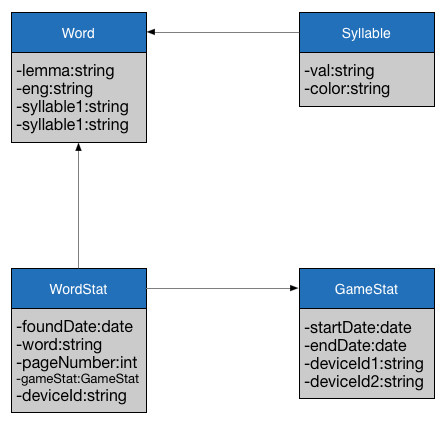
\includegraphics[width=\textwidth]{entities.png}}
  \caption{Entità presenti nel database}
\end{figure}

\section{Inizializzazione}
Il database viene inizializato la prima volta che l'applicazione viene aperta con i dati in formato \textit{JSON} presenti nei files \code{words.json} e \code{syllable.json} contenuti nella cartella degli \code{assets}.\\
Il listing \ref{lst:words_json} contiene un estratto del file \code{words.json}

\begin{lstlisting}[float, caption=Porzione del file \code{words.json}, label=lst:words_json]
[
  {
    "lemma":"arco",
    "eng":"arc",
    "syllable1":"ar",
    "syllable2":"co"
  },
  ...
\end{lstlisting}

Il mapping degli elementi JSON con la classe Java associata avviene tramite la libreria Open Source GSON, sviluppata da Goolge, che fa uso di annotazioni per mappare gli attributi delle classi con i campi JSON.\\
L'operazione di conversione dei dati da JSON a classi Java e il successivo inserimento all'interno del database, in quanto operazioni relativamente lunghe, non vengono eseguite all'interno del \textit{Thread} principale ma in uno differente grazie ad un \code{IntentService} contenuto in \\\code{it.gbresciani.legodigitalsonoro.services.InitDBService}. 

